\section{Ля}
\label{section:audio feature extraction} % это сами поменяете

А тут рисуночек будет...
\ref{fig:sg_of_key}.

\begin{figure}[ht]
    \centering
    \vspace{0ex}
    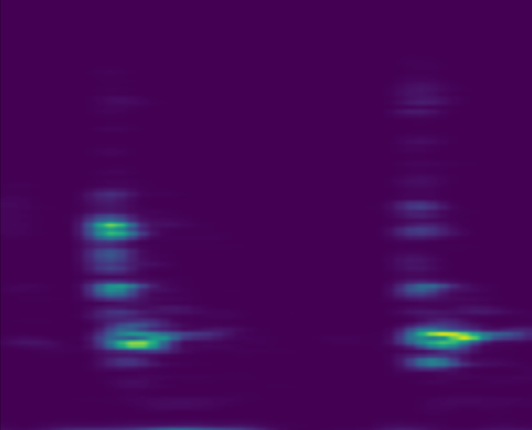
\includegraphics[width=0.5\linewidth]{imgs/mel_spec_key.png}
    \caption{Пример спектрограммы звука нажатия клавиши}
    \label{fig:sg_of_key}
\end{figure}

А тут ссылочка \cite{Abdul_Jamil:Speech Emotion Recognition} 


\section{Траляля}

\subsection{Ля тополя}

А тут формулка:
\begin{equation}
V = \sum_{i=1}^{k} \sum_{x \in S_i} (x - \mu_i)^2,
\label{eq:k-means min}
\end{equation}

где k -- число кластеров,

\hspace{1.5em}$S_{i}$ -- полученные кластеры,

\hspace{1.6em}$i=1,2,\dots ,k$,

\hspace{1.5em}$\mu _{i}$ -- центры масс всех векторов $x$ из кластера $S_{i}$.

Ляляляляллялялл

А тут ссылочка на формулку: \ref{eq:k-means min}.

\subsection{аоаодолд}
Труляля тут перечисление:
\begin{description}[font=\normalfont\itshape{- } ]
    \item[Внешние меры оценки качества.] Данные меры используют дополнительные знания о кластеризуемом множестве: распределение по кластерам, количество кластеров и т.д..
    \item[Внутренние меры оценки качества.] Данные меры оценивают качество структуры кластеров опираясь только непосредственно на нее, не используя внешней информации.
\end{description}


% Добавить источники для алгоритмов
Еще перечислим что-то:
\begin{itemize}[]
    \item и раз,
    \item и два,
    \item и три.
\end{itemize}

И на всякий еще что-то перечислим, но ссылочками:
\begin{itemize}[]
    \item и раз \cite{Calinski  Harabas: cluster analysis},
    \item и два \cite{Peter J. Rousseeuw. Silhouettes}.
\end{itemize}

\section{Труляля}

А тут что-то на математическом:

Пусть $X \in \mathds{R}^N$ -- множество размерности $N$, тогда преобразование $a : X \in \mathds{R}^N \rightarrow Y \in \mathds{R}^M$ , где $M<N$ -- преобразование снижения размерности.

Еще перечислим: 
\begin{description}[font=\normalfont\itshape{- } ]
    \item[Отбор признаков.] Отбираем.
    \item[Выделение признаков.] Выделяем.
\end{description}

\subsection{Ща еще что-то вставим (куда-то или кому-то)}
ЩА будет формулка..

Метод состоит в поиске $n$ главных компонент множества точек \linebreak $x_1, x_2, \dots, x_m \in\mathbb{R}^n$. Первая главная компонента -- это такая линия $L_n$, для которой выполняется условие:
\begin{equation}
\sum_{i=1}^m \operatorname{dist}^2(x_i, L_n) \to \min.
\label{eq:pca min}
\end{equation}


Еще перечислим:

\begin{enumerate}[label=\arabic*)]
    \item Раз: 
    \begin{equation}
    x_i := x_i - \overline{X}.
    \label{eq:pca1}
    \end{equation}
    
    Теперь $\sum_{i=1}^m x_i =0.$
    \item Два:
    \begin{equation}
    a_1 = \underset{\Vert a_1 \Vert =1}{\operatorname{argmin}} \left( \sum_{i=1}^m \Vert x_i - a_1 (a_1,x_i)\Vert ^2\right).
    \label{eq:pca2}
    \end{equation}
    если решение не единственно, то осуществляется выбор одного из них.
    
    \item Три:
    \begin{equation}
    x_i := x_i - a_1 \left(a_1,x_i\right).
    \label{eq:pca3}
    \end{equation}
    
    \item Четыре: 
    \begin{equation}
    a_2 = \underset{\Vert a_2 \Vert =1}{\operatorname{argmin}} \left( \sum_{i=1}^m \Vert x_i - a_2 (a_2,x_i)\Vert ^2\right).
    \label{eq:pca4}
    \end{equation}
    
\end{enumerate}

Формулка:
\begin{equation}
a_k = \underset{\Vert a_k \Vert =1}{\operatorname{argmin}} \left( \sum_{i=1}^m \Vert x_i - a_k (a_k,x_i)\Vert ^2\right).
\label{eq:pca5}
\end{equation}

\subsection{Ляляляля}

Щас еще перечислим. 
\begin{enumerate}[label=\arabic*)]
    \item Раз.
    \item Два.
\end{enumerate}

Ссылка на рисуночек тут \ref{fig:crisp_dm}.
Тут я че-то не поняла как оно, но разберетесь

\begin{figure}[ht]
    \centering
    \vspace{0ex}
    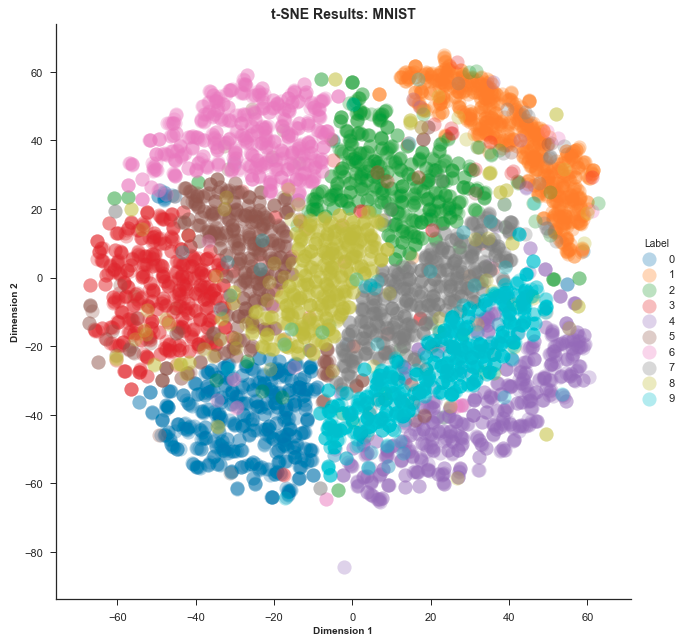
\includegraphics[width=0.7\linewidth]{imgs/tsneMNIST.png}
    \caption{Визуализация MNIST с помощью t-SNE}
    \label{fig:crisp_dm}
\end{figure}


Перечислим:

\begin{itemize}[]
    \item Раз.
\end{itemize}

\begin{itemize}[]
    \item Два.
\end{itemize}

\subsection{Ляляляляля}

\section{Ля}

Перечислим с чиселками:
\begin{enumerate}[label=\arabic*)]
    \item Раз.
    \item Два.
\end{enumerate}























